\chapter{Related Work}
\label{cha:relatedwork}

The following chapter covers the most significant concepts required to comprehend this thesis's approach. It includes a closer look at decentralized communication protocols, identifier standards, and social networks that implement them. The revision and structuring of these concepts allow us to understand, build upon, and apply them to address our identified research questions.

\section{Social Web Protocols}
Between 2014 and 2018, the Social Web Working Group (SocialWG) from the W3C embarked on the journey to bring social-networking standards to the Web. This journey included defining technical protocols, vocabularies, and APIs focusing on social interactions. Following the idea that systems implementing these features should be able to communicate with each other in a decentralized manner. These four years resulted in several W3C Recommendations, including a collection of standards that enable various aspects of decentralized social web interaction called \emph{Social Web Protocols} \cite{celik_prodromou_le_hors_2014}. Standards found in this collection are \emph{WebSub}\footnote{https://www.w3.org/TR/websub/}, \emph{WebMention}\footnote{https://www.w3.org/TR/webmention/}, \emph{Linked Data Notifications}\footnote{https://www.w3.org/TR/ldn/}, and the two most relevant for this thesis, \emph{ActivityStreams 2.0}\footnote{https://www.w3.org/TR/activitystreams-core/} and \emph{ActivityPub}\footnote{https://www.w3.org/TR/activitypub/}.

% ------------ActivityStreams------------------------------------
\subsection{ActivityStreams 2.0}\label{subsec:activitystreams}

% First, it is essential to be able to describe an \emph{Activity}. 

ActivityStreams 2.0 is a standard that provides a model for representing \emph{Activities} using a JSON-based syntax. Additionally, it provides a vocabulary that includes all the standard terms needed to represent social activities \cite{snell_prodromou_2017}. This standard describes an activity following a story of an \emph{actor} performing an \emph{action} on an \emph{object}. It specifies different types of actors, activities, and objects, as shown in \autoref{table:activitystreams_vocabulary}. Each of these objects can be represented as a JSON object, creating a solid foundation upon which other protocols can build. 

\begin{table}[H]
  \centering
  \begin{tabular}{|p{4cm}|p{4cm}|p{4cm}| }
    \hline
    \multicolumn{3}{|c|}{ActivityStreams Vocabulary} \\
    \hline
    \textbf{Activity types} & \textbf{Actor types} & \textbf{Object types} \\
    \hline
    \hline
      Accept, Add & Application & Note \\ 
      Announce, Arrive & Group & Document \\ 
      Block, Create & Organization & Image \\
      Delete, Dislike & Person & Article \\
      Flag, Follow & Service & Profile \\
      Ignore, Invite & & Audio \\
      Join, Leave & & Event \\
      Like, Listen & & Tombstone \\
      \hline
  \end{tabular}
  \caption{ActivityStreams 2.0 vocabulary examples}
  \label{table:activitystreams_vocabulary}
\end{table}

ActivityStreams 2.0 has improved its 1.0 version in more than one aspect. One of these is the compatibility with JSON-LD\footnote{https://www.w3.org/TR/json-ld/}, which is a JSON serialization for \emph{Linked Data}\footnote{https://www.w3.org/DesignIssues/LinkedData.html}. The concept of Linked Data is based on interlinking data in such a way that it becomes more usable through associative and contextual queries \cite{berners-lee_2006}.\. With JSON-LD, ActivityStreams 2.0 can define its own context and the terms that will be used inside this context. Listing \ref{fig:activitystream_example} shows an example of a JSON-LD serialized ActivityStreams 2.0 activity. 

\lstset{style=JSONStyle}
\begin{lstlisting}[language=PHP, caption=Example of a Create activity using JSON-LD \cite{snell_prodromou_2017}, label=fig:activitystream_example, float=h]
  {
    "@context": "https://www.w3.org/ns/activitystreams",
    "summary": "Alice created an image",
    "type": "Create",
    "actor": "http://www.test.example/Alice",
    "object": "http://example.org/foo.jpg"
  }
\end{lstlisting}

% ------------ActivityPub------------------------------------
\subsection{ActivityPub}\label{subsec:activitypub}

ActivityPub is another W3C Recommendation that originated from the SocialWG. It is a decentralized social networking protocol that is based on the syntax and vocabulary of ActivityStreams 2.0. It provides a client-to-server API, which covers the requirements of a Social API\cite{guy_2017}, i.e., publishing, subscribing, reading content, and notifying when content gets created. In addition, it provides a server-to-server API that enables federated communication. Furthermore, it provides users with a JSON-based \emph{profile}, which is an ActivityStreams 2.0 actor object. This actor object includes standard properties such as \emph{name}, \emph{type}, and \emph{summary}. ActivityPub extended this actor object with several properties. Extended optional properties include collections such as \emph{following, followers}, and \emph{liked}. Compulsory properties include an \emph{inbox} and an \emph{outbox}. These last two URLs represent how the actor gets and sends messages from other users. Listing \ref{fig:actor_object} shows an example of an ActivityPub object with the extended properties. 


%  Actor Object ActivityPub
\lstset{style=JSONStyle}
\begin{lstlisting}[language=PHP, caption=Actor object example in ActivityPub \cite{lemmer-webber_tallon_guy_prodromou_2018}, label=fig:actor_object, float=h!]
  {
    "@context": "https://www.w3.org/ns/activitystreams",
    "type": "Person",
    "id": "https://social.example/alice/",
    "name": "Alice P.",
    "preferredUsername": "alice",
    "summary": "TU Berlin student",
    "inbox": "https://social.example/alice/inbox/",
    "outbox": "https://social.example/alice/outbox/",
    "followers": "https://social.example/alice/followers/",
    "following": "https://social.example/alice/following/",
    "liked": "https://social.example/alice/liked/"
  }
\end{lstlisting}

There are two workflows of communication for a user in ActivityPub, as shown in figure \ref{fig:ap_flow} \label{subsec:ap_workflows}

\begin{itemize}
  \item \textbf{Client-to-Server Communication:} A user wants to share a post publicly. This requires an HTTP POST request to his outbox with the respective activity object. After this, other users interested in seeing this user's post can make an HTTP GET request to the user's outbox and retrieve it.
  \item \textbf{Server-to-Server Communication (Federation)}: User \emph{A} wants to send a post to user \emph{B}, whose account is on a different server. For this scenario, the following steps are required. First, user \emph{A} posts his message to his outbox. Consequently, his server looks for \emph{B}'s inbox and performs an HTTP POST request. Finally, \emph{B} makes an HTTP GET request to his inbox to retrieve all the posts addressed to him.
  
  A key thing to remember is that for this type of communication, \emph{A}'s server has to retrieve somehow the \emph{inbox} of user \emph{B} based only on his username. This resolving process is not part of the ActivityPub specification. Therefore, implementers of this standard must find a way to achieve this independently. 
\end{itemize}
 

\begin{figure}[H]
  \centering
  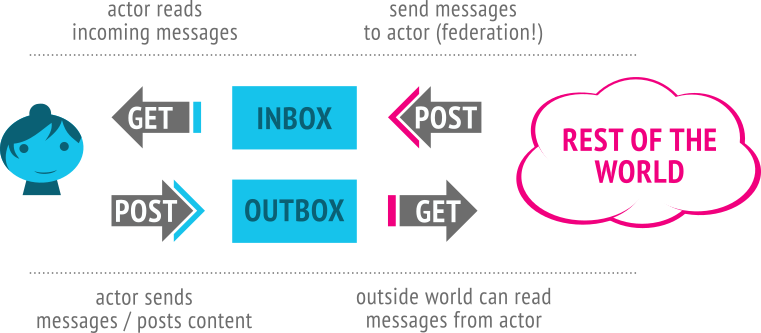
\includegraphics[width=0.8\textwidth]{related_work/ActivityPub-tutorial-image.png}
  \caption{ActivityPub overview \cite{lemmer-webber_tallon_guy_prodromou_2018}}
  \label{fig:ap_flow}
\end{figure}


Regarding security, although ActivityPub's specification does not define any official security mechanisms, it mentions a list published by the SocialWG of best security practices\footnote{https://www.w3.org/wiki/SocialCG/ActivityPub/Authentication\_Authorization} that may be used in an ActivityPub implementation. This list suggests using standards such as OAuth 2.0\footnote{https://oauth.net/2/} for client-to-server authentication, as well as HTTP Signatures\footnote{https://tools.ietf.org/html/draft-cavage-http-signatures-08} and Linked Data Signatures\footnote{https://w3c-dvcg.github.io/ld-signatures/} for server-to-server authentication. Furthermore, it recommends using HTTPS for its HTTP-based communication to provide transport-layer encryption.


% ------------ActivityPub-Based social networks------------------------------------
\section{ActivityPub-based Social Networks}

\subsection{The Fediverse}

It is impossible not to refer to the \emph{Fediverse} when ActivityPub is mentioned. The \emph{Fediverse} is an interoperable collection of different federated social networks running on free open software on thousands of servers across the world that implement the same open-standard protocols to be able to interact with each other. It is developed by a not-profit-driven community of people around the globe independent of any corporation or official institution \cite{holloway_2018} \cite{https://doi.org/10.48550/arxiv.1909.05801}. The simplest way to explain how the federation works is the following example: Bob has a Twitter account, which he uses to follow all his friends that also have a Twitter account. Alice is a friend of Bob, but she only has an account on Youtube. In the real world, these two services are completely isolated and cannot communicate. However, if both had implemented the same social network protocol, such as ActivityPub, Bob would be able to find Alice by a normal search on Twitter and follow her. Allowing any new post of Alice on Youtube, to appear in Bob's Twitter timeline.

Before ActivityPub, the \emph{Fediverse} implemented other protocols like \emph{Ostatus}\footnote{https://ostatus.github.io/spec/OStatus\%201.0\%20Draft\%202.html}, \emph{Matrix}\footnote{https://matrix.org}, and \emph{Diaspora}\footnote{https://diaspora.github.io/diaspora\_federation}. However, after ActivityPub was published as a Recommendation by the SocialWG in January 2018, many of these federated social networks upgraded to ActivityPub, becoming the predominant protocol rapidly. Furthermore, the range of services that can be found inside the \emph{Fediverse} includes blogging, microblogging, video streaming, photo, music sharing as well as file hosting. Examples are shown in table \ref{table:fediverse_examples}.

\begin{table}[H]
  \centering
  \begin{tabular}{|p{4cm}|p{4cm}|p{4cm}| }
    \hline
    \textbf{Name} & \textbf{Type} & \textbf{
      Equivalent to} \\
    \hline
    \hline
    \textbf{\footnote{https://joinpeertube.org}PeerTube} & Video sharing  & Youtube \\
    \textbf{\footnote{https://friendi.ca}Friendica} & Social networking & Facebook \\ 
    \textbf{\footnote{https://joinmastodon.org}Mastodon} & Microblogging & Twitter \\
    \textbf{\footnote{https://pixelfed.org}Pixelfed} & Photo sharing & Instagram \\
      \hline
  \end{tabular}
  \caption{Examples of DOSN in the Fediverse}
  \label{table:fediverse_examples}
\end{table}

% \begin{itemize}
%   \item \textbf{PeerTube\footnote{https://joinpeertube.org}:} A decentralized alternative to , similar to Youtube.
%   \item \textbf{Friendica\footnote{https://friendi.ca}:} A Facebook-like DOSN.
%   \item \textbf{Mastodon\footnote{https://joinmastodon.org}:} Microblogging platform, similar to Twitter.
%   \item \textbf{Pixelfed\footnote{https://pixelfed.org}:} An image-sharing platform, similar to Instagram. 
% \end{itemize} 

Although it was not the first social network to implement ActivityPub, Mastodon is the one that pioneered its use on a large scale \cite{lemmer-webber_2017}. In addition, it is the DOSN in the \emph{Fediverse} with the most extensive user base and popularity. For this reason, Mastodon will be used in this thesis to represent the ActivityPub-based social networks and will be explained further in the next section. 

% ------------Mastodon------------------------------------
\subsection{Mastodon}\label{subsec:mastodon}

 Mastodon is a decentralized Twitter-like microblogging social network created with the idea of bringing social networking back into the hands of its users. The german creator of Mastodon, Eugen Rochko, shared the same opinion as what Fitzpatrick and Recordon said in 2007 \cite{fitzpatrick_recordon_2007}: \emph{People are getting sick of registering and re-declaring their friends on every site}. For this reason, Eugen envisioned a social network that could end this, and \emph{last forever} \cite{tilley_2018}. Like the \emph{Fediverse}, Mastodon differs from other commercial social networks in two aspects. First, it is oriented towards small communities and community-based services. Each \emph{instance}\footnote{A server running Mastodon} is free to choose its topics; this way, users are encouraged to choose the instance better suited to their taste. Second, the Mastodon platform eliminates the presence of sponsored users or posts in feeds. This implies that the only way to connect or consume content is through a self-search to find an already known account or to explore the users' feeds in other instances with similar interests \cite{8845221}. 
 
 From a user experience perspective, Mastodon includes all the essential features of a microblogging platform, such as:

\begin{itemize}
  \item Follow other users, even if they are not in the same instance. 
  \item Post small status updates, or \emph{toots}, up to 500 characters long. 
  \item Access to a timeline of the local instance and federated statuses. 
  \item Control over the visibility of their posts, with the option to set them as private, instance-level only, or federated. 
\end{itemize}

Mastodon's implementation of ActivityPub follows the guidelines defined by the spec. However, as the protocol does not specify how to implement some key processes required for a fully-working social network, Mastodon extended the protocol with the following processes and features.

\subsubsection*{\textbf{Security}}
Mastodon implemented the authentication and authorization mechanisms from the best practices list of the SocialWG to address the security concerns in ActiviyPub. The ones relevant to this thesis are the HTTP and the JSON-LD signatures. HTTP signatures extend the HTTP protocol by adding the possibility to sign the HTTP requests cryptographically. This signature gets added to the request within the \emph{Signature} header, and it provides not only end-to-end message integrity but also proof of the authenticity of the sender without the need for multiple round-trips \cite{cavage_sporny_2019}. Creating an HTTP signature means signing the parameters of the request itself, i.e the \emph{request-target}, the \emph{host}, and the \emph{date}. These parameters and their values are concatenated in a single string, hashed, and signed with the sender's public key. Finally, the \emph{Signature} header indicates the key used to sign the document, the parameters inside the signature, and the algorithm used to hash it. An example in Mastodon is shown by listing \ref{fig:http_signature}. 
Following the same idea, Linked Data Signatures offer a way to create and attach signatures to JSON-LD documents. This kind of signature can provide non-repudiation to a JSON-LD object, like an ActivityStreams Activity object, even if the object has been shared, forwarded, or referenced at a future time \cite{celik_prodromou_le_hors_2014}. However, this feature, although implemented, is not actively used in Mastodon. For Mastodon to be able to implement these signatures, it was necessary to generate keypairs for the users. For this reason, Mastodon added a new property \emph{publicKey} to the actor object, which includes the pem-formatted public key of an RSA-2018 keypair. See appendix \ref{fig:mastodon_actor_object} for the complete actor object that includes the added properties in the Mastodon implementation.

\lstset{style=JSONStyle}
\begin{lstlisting}[language=PHP, caption=Signed HTTP Request, label=fig:http_signature, float=h]

GET /users/username/inbox HTTP/1.1
Host: mastodon.example
Date: 18 Dec 2019 10:08:46 GMT
Accept: application/activity+json
Signature: keyId="https://my-example.com/actor#main-key",headers="(request-target) host date",signature="Y2FiYW...IxNGRiZDk4ZA=="

\end{lstlisting}

\subsubsection*{\textbf{Resolving accounts}}
As explained in \ref{subsec:ap_workflows}, ActivityPub requires a resolving process when sending a message to a user whose account resides on a different server. For this, Mastodon implemented \emph{Well-Known URIs}\footnote{https://www.rfc-editor.org/rfc/rfc8615.html}, which enable the discovery of information about an origin in well-known endpoints \cite{nottingham_2019}. The two most relevant endpoints are the following: 

\subsubsection*{Web Host Metadata}
This endpoint allows the discovery of host information using a lightweight metadata document format. In this context, \emph{host} refers to the entity in charge of a collection of resources defined by URIs with a common URI host \cite{cook_2011}. It employs the XRD 1.0\footnote{https://docs.oasis-open.org/xri/xrd/v1.0/os/xrd-1.0-os.html} document format, which offers a basic and flexible XML-based schema for resource description. Moreover, it provides two mechanisms for providing resource-specific information, \emph{link templates} and \emph{Link-based Resource Descriptor Documents} (LRDD). On the one hand, link templates require a URI to work, thus avoiding the use of fixed URIs. On the other hand, the LRDD relation type is used to relate \emph{LRDD documents} to resources or host-meta documents \cite{cook_2011}. In the specific case of the Mastodon implementation, requesting the host-meta endpoint will give us back the \emph{lrdd} link to the Webfinger endpoint, where specific resource information can be found. This is illustrated by figures \ref{fig:host_metadata_response} and \ref{fig:host_metadata_request}.

\lstset{style=JSONStyle}
\begin{lstlisting}[language=PHP, caption=Web Host Metadata request to mastodon.social, label=fig:host_metadata_request, float=ht]
    GET /.well-known/host-meta HTTP/1.1
    Host: mastodon.social
    Accept: application/xrd+xml
\end{lstlisting}

\lstset{style=JSONStyle}
\begin{lstlisting}[language=XML, caption=Web Host metadata response from mastodon.social, label=fig:host_metadata_response, float=h!]
    <?xml version="1.0" encoding="UTF-8"?>
    <XRD xmlns="http://docs.oasis-open.org/ns/xri/xrd-1.0">
      <Link rel="lrdd" template="https://mastodon.social/.well-known/webfinger?resource={uri}"/>
    </XRD>
\end{lstlisting}

\subsubsection*{\textbf{Webfinger}}
Mastodon relies on the Webfinger protocol for the resolving process and its federated functioning \cite{rochko_2020}. It is an HTTP-based protocol that allows for discovering information about persons or other entities on the Internet. This information can be a personal profile, an address, an identity service, a telephone number or an email \cite{jones_salgueiro_jones_smarr_2013}. Performing a query to a WebFinger endpoint requires a query component with a resource parameter, which is the URI that identifies the identity that is being looked up. Mastodon employs the \emph{acct}\footnote{https://datatracker.ietf.org/doc/html/rfc7565} URI format, which aims to offer a scheme that generically identifies a user's account with a service provider without requiring a specific protocol. Webfinger's response consists of a \emph{JSON Resource Descriptor} (JRD) document describing the entity \cite{jones_salgueiro_jones_smarr_2013}. Fig. \label{Webfinger response from mastodon.social} shows an example of the returned JRD document provided by the WebFinger endpoint of the \emph{mastodon.social}\footnote{https://mastodon.social} instance when querying the account \emph{acct:bob@mastodon.social}.

\lstset{style=JSONStyle}
\begin{lstlisting}[language=PHP, caption=HTTP request to Webfinger endpoint, label=Webfinger request, float=h]
  GET /.well-known/webfinger?resource=acct:bob@mastodon.social
  Host: mastodon.social
  Accept: application/xrd+xml
\end{lstlisting}

\lstset{style=JSONStyle}
\begin{lstlisting}[language=PHP, caption=Webfinger response, label=Webfinger response from mastodon.social, float=h]
{
   "subject": "acct:bob@mastodon.social",
   "aliases": [
       "https://mastodon.social/@bob",
       "https://mastodon.social/users/bob"
   ],
   "links": [
       {
           "rel": "http://webfinger.net/rel/profile-page",
           "type": "text/html",
           "href": "https://mastodon.social/@bob"
       },
       {
           "rel": "self",
           "type": "application/activity+json",
           "href": "https://mastodon.social/users/bob"
       },
   ]
}
\end{lstlisting}


\pagebreak
% ------------Extending ActivityPub------------------------------------
\section{Extending ActivityPub}\label{sec:extending_activitypub}

This thesis is not the first attempt to address the deficiencies of the ActivityPub protocol. The co-author of ActivityPub, Christopher Webber, and the co-author of the DID specification Manu Sporny presented a different approach during the Rebooting Web of Trust\footnote{https://www.weboftrust.info/} summit in 2017 \cite{webber_sporny_2017}. This approach includes the following features:

\subsection*{\textbf{End-To-End Encryption}}\label{subsec:e2e}

To create a web of trust when using ActivityPub, the authors suggested using the IETF standard OpenPGP\footnote{https://www.openpgp.org/}, which provides a format for encrypting data using public key cryptography. This way, only the user's device that contains the private key can decrypt and read the plain-text message. However, this encryption brings a series of consequences that affect the usability of a social network. Especially on the server side, some \emph{activities} trigger callbacks that the server usually processes in the background. For example, if a server receives a \emph{like} activity, it will increase a counter, add the liked post to the \emph{liked} collection, and notify the post's creator. Nevertheless, all these features cannot be performed if the activity is encrypted. Other consequences include the key management for the users, which makes the user experience problematic, and in case of key loss, there would be no way to read old posts \cite{webber_sporny_2017}. Listing \ref{lst:ap_encrypted} shows an example of an encrypted Activity.

\lstset{style=JSONStyle}
\begin{lstlisting}[language=PHP, caption=Note object with encrypted content \cite{webber_sporny_2017}, label=lst:ap_encrypted, float=h]
{
  "@context": ["https://securityns.example/",
  "https://www.w3.org/ns/activitystreams"],
  "type": "EncryptedEnvelope",
  "encryptedMessage": "-----BEGIN PGP MESSAGE-----\r\n...",
  "mediaType": "application/ld+json; profile=\"https://www.w3.org/ns/activitystreams\"
}
\end{lstlisting}

\subsection*{\textbf{Signing Objects}}
They proposed using JSON-LD signatures to provide non-repudiation and to assert the integrity of messages sent over the network. They added a public key property to the actor object, just as Mastodon did to enable HTTP Signatures. The resulting signed activity is shown by listing \ref{lst:signed_activity}.

\lstset{style=JSONStyle}
\begin{lstlisting}[language=PHP, caption=Note object with JSON-LD Signature. Adapted from \cite{webber_sporny_2017}, label=lst:signed_activity, float=h]
  {
    "type": "Note",
    "id": "https://social.example/alyssa/posts/63cc87ec-416e-437d-...",
    "attributedTo": "https://social.example/alyssa/",
    "to": ["https://havoc.example~mallet/"],
    "content": "Tortellini are delicious",
    "signature": {
      "type": "RsaSignature2017",
      "creator": "https://social.example/alyssa/",
      "created": "2017-09-23T20:21:34Z",
      "nonce": "e3689a56da9b4bc",
      "signatureValue": "mJfe5OCb7J3WwI...8t5/m="
      }
  }
\end{lstlisting}

\subsection*{\textbf{Introducing DIDs}}
Their approach to implementing DIDs is using DIDs as actors. Thus, switching from a standard URL like \emph{https://social.example/alyssa/} to a DID. 

\subsection*{\textbf{Integrating ActivityPub into the DID document}}

The authors opted to combine the actor object into the DID document, allowing all the necessary endpoints to be discoverable and stored in the VDR. In addition, to remove any dependency on a centralized DNS, the inbox, outbox, following, and other properties are now based on Tor Hidden Services\footnote{https://www.torproject.org}. The resulting DID document is illustrated by listing \ref{lst:did_and_ap}

\lstset{style=JSONStyle}
\begin{lstlisting}[language=PHP, caption=DID document with inserted ActivityPub actor. Adapted from \cite{webber_sporny_2017}, label=lst:did_and_ap, float=h]
  {
    "@context": ["https://example.org/did/v1",
                 "https://www.w3.org/ns/activitystreams"],
    "id": "did:example:d20Hg0teN72oFeo0iNYrblwqt",
    "activityPubService": {
      "id": "did:example:d20Hg0teN72oFeo0iNYrblwqt#services/ActivityPub",
      // ActivityPub actor information
      "type": "Person",
      "name": "Alyssa P. Hacker",
      "preferredUsername": "alyssa",
      "summary": "Lisp enthusiast hailing from MIT",
      "inbox": "https://9GaksjPhy0mWToTV.onion/alyssa/inbox/",
      "outbox": "https://9GaksjPhy0mWToTV.onion/alyssa/outbox/",
      "followers": "https://9GaksjPhy0mWToTV.onion/alyssa/followers/",
      "following": "https://9GaksjPhy0mWToTV.onion/alyssa/following/",
      "liked": "https://9GaksjPhy0mWToTV.onion/alyssa/liked/"},
    // DDO information
    "owner": [{
      "id": "did:example:d20Hg0teN72oFeo0iNYrblwqt#key-1",
      "type": ["CryptographicKey", "EdDsaPublicKey"],
      "curve": "ed25519",
      "expires": "2017-02-08T16:02:20Z",
      "publicKeyBase64": "lji9qTtkCydxtez/bt1zdLxVMMbz4SzWvlqgOBmURoM="
    }],
    "control": [{
      "type": "OrControl",
      "signer": [
          "did:example:d20Hg0teN72oFeo0iNYrblwqt",
          "did:example:8uQhQMGzWxR8vw5P3UWH1j"
      ]
    }],
    "created": "2002-10-10T17:00:00Z",
    "updated": "2016-10-17T02:41:00Z"
  }
\end{lstlisting}


Mastodon implemented another approach to extending ActivityPub, which consists of an end-to-end encryption API\footnote{https://github.com/mastodon/mastodon/pull/13820}. This API was the result of a long-discussed feature request\footnote{https://github.com/mastodon/mastodon/issues/1093} for an Off-The-Record\footnote{https://otr.im/}  (OTR) endpoint for direct messages. In this discussion, different alternatives were mentioned, such as using the PGP-based Mailvelope\footnote{https://mailvelope.com/en}, which provides end-to-end mail encryption; or the Message Layer Security (MLS)\footnote{https://datatracker.ietf.org/doc/draft-ietf-mls-protocol/} from the IETF. In the end, they added an API to send messages using the Matrix\footnote{https://matrix.org/docs/projects/other/olm} implementation of the Double Ratchet Algorithm\footnote{https://signal.org/docs/specifications/doubleratchet/}, which is part of the protocol used in the messaging app Signal\footnote{https://signal.org}. With these endpoints, it is possible to register a device with a key generated by Mastodon and to send encrypted messages to specific devices of other people.

This implementation follows the same idea proposed by Webber and Sporny in \ref{subsec:e2e}. Nonetheless, it is still unclear why Mastodon has kept this feature \emph{hidden}. There is no documentation, and designing a UI for it is not planned. Therefore, preventing people from knowing and taking advantage of it. For an example of an encrypted Activity using this endpoint see appendix \ref{appendix:e2e}. 

% ------------DIDs------------------------------------
\section{Decentralized Identifiers} \label{section:dids}

On July 19. 2022 the W3C announced that Decentralized Identifiers (DIDs) v1.0 is officially a Web standard. This new type of globally unique identifier brings a Self-Sovereign approach to digital identities, enabling individuals and organizations to take control of their online information and relationships while also providing greater security and privacy \cite{w3c_2022}. Self-Sovereign Identity \emph{SSI} implies a sovereign, enduring, decentralized, and portable digital identity for any human or non-human entity that enables its owner to access services in the digital world in a secure, private, and trusted manner. DIDs are the key component of the SSI framework, as they allow identifiers to be created independently of any centralized registry, identity provider, or certificate authority with full control given to its owner\cite{Naik_Jenkins_2021}\cite{sporny_longley_sabadello_reed_steele_2021}.

\subsection{Architecture}

The DID itself is a URI that consists of 3 different parts. The DID URI scheme identifier, the method identifier, and the DID method-specific identifier as shown in figure \ref{fig:did}. The entity being identified by the DID is called the \emph{DID subject}. \emph{Everything} can be identified by a DID, including any person, group, organization, as well as a physical, digital, or logical thing \cite{Conway_Hughes_Ma_Poole_Riedel_2019}\cite{sporny_longley_sabadello_reed_steele_2021}.

\begin{figure}[h]
  \centering
  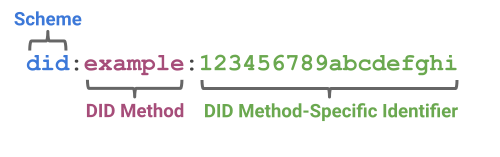
\includegraphics[width=0.5\textwidth]{related_work/parts-of-a-did.png}
  \caption{DID composition \cite{sporny_longley_sabadello_reed_steele_2021}}
  \label{fig:did}
\end{figure}


The DID Subject that can modify the DID Document is called the \emph{DID controller}. Usually, the DID subject is the DID controller, but this is not compulsory. As shown in figure \ref{fig:did_architecture}, a DID resolves to a \emph{DID Document}, which is a JSON-based object that contains information associated with a DID. It includes verification methods, such as cryptographic public keys and relevant services to interact with the DID Subject. An example of a DID Document can be seen in \ref{fig:did_document}. Furthermore, it is possible to retrieve a specific resource of the DID document by using a \emph{DID URL}, which is a DID that includes a path, query, or fragment \cite{sporny_longley_sabadello_reed_steele_2021}.

% ---- DID Document -----
\lstset{style=JSONStyle}
\begin{lstlisting}[language=PHP, caption=Example DID Document, label=fig:did_document]

{
  "@context": "https://w3id.org/did/v1",
  "id": "did:example:123456789abcdefghi",
  "publicKey": [{
    "id": "did:example:123456789abcdefghi#keys-1",  // DID URL 
    "type": "RsaVerificationKey2018",
    "owner": "did:example:123456789abcdefghi",
    "publicKeyPem": "..."
  }],
  "authentication": [{
    "type": "RsaSignatureAuthentication2018",
    "publicKey": "did:example:123456789abcdefghi#keys-1"
  }],
  "service": [{
    "type": "ExampleService",
    "serviceEndpoint": "https://example.com/endpoint/8377464"
  }]
}

% \end{lstlisting}
 
DID documents are stored in a \emph{Verifiable Data Registry} (VDR). A VDR is essentially any system that enables capturing DIDs and returning required data to generate DID documents. For example, distributed ledgers, decentralized file systems, any decentralized database, peer-to-peer networks, or other types of trustworthy data storage. The next component is the \emph{DID method}, which describes the processes for CRUD operations for DIDs and DID documents based on a specific type of VDR. According to the DID registry\footnote{https://www.w3.org/TR/did-spec-registries/\#did-methods} of the W3C, there are around 103 registered DID method specifications. More information about the different existing DID methods can be found in \autoref{subsec:did_methods}.

The last major component in this architecture overview is the one in charge of resolving DIDs, namely, the \emph{DID resolver}. This component implements the \emph{DID resolution}, which consists of taking a DID as an input, and giving a DID Document as an output \cite{sporny_longley_sabadello_reed_steele_2021}. The Identifiers \& Discovery Working Group (ID WG) has implemented a prototype Universal Resolver\footnote{https://github.com/decentralized-identity/universal-resolver}, which allows the resolution of DIDs for numerous DID methods. In addition, this working group has also developed a Universal Registrar\footnote{https://uniregistrar.io/}, which allows the creation, edition, and deactivation of the DIDs across different DID methods.

\begin{figure}[H]
  \centering
  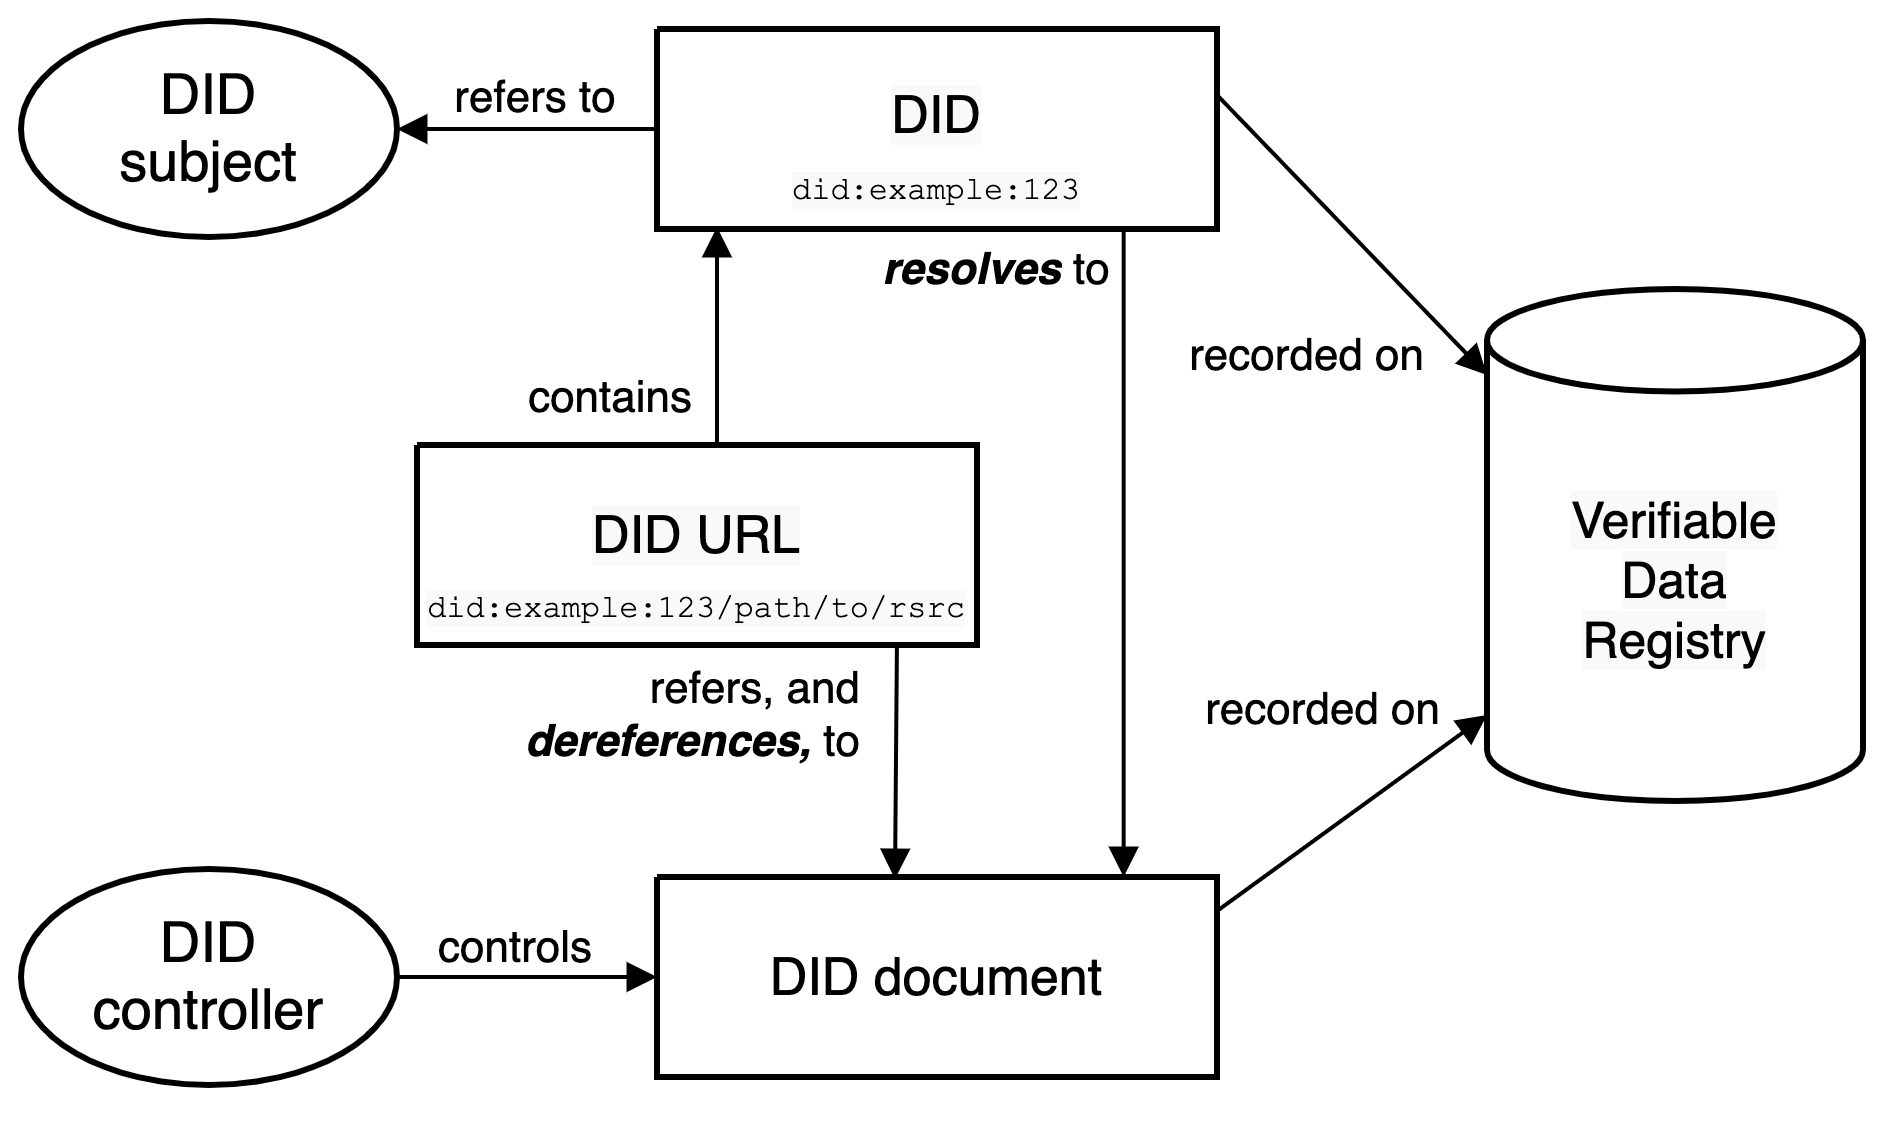
\includegraphics[width=0.8\textwidth]{related_work/did_brief_architecture_overview.png}
  \caption{DID architecture overview \cite{sporny_longley_sabadello_reed_steele_2021}}
  \label{fig:did_architecture}
\end{figure}

\subsection{DID methods}\label{subsec:did_methods}

 Based on their characteristics and patterns, most DIDs can be sorted into different categories \cite{preukschat_reed_2021}, for example: 

\begin{itemize}
  \item \textbf{Ledger-based DIDs}: This includes all the DIDs that store DIDs in a blockchain or other Distributed Ledger Technologies (DLTs). Examples include \emph{did:btcr}, \emph{did:ethr} and \emph{did:trx}, whose DIDs are stored in the Bitcoin, Ethereum, and Tron network respectively.
  \item \textbf{Ledger Middleware (\emph{Layer 2}) DIDs}: Layer 2 refers to a framework or protocol that is built on top of an existing blockchain system that takes the transactional burden away from layer 1, making it more scalable \cite{weston_2022}. An example DID method in this category is the \emph{did:ion}\footnote{https://identity.foundation/ion/}, which runs in a layer on top of Bitcoin. 
  \item \textbf{Peer DIDs}: DIDs have the required ability to be resolvable. However, not all of them have to be globally resolvable. Peer DIDs do not exist on a global source of truth but in the context of relationships between peers in a limited number of participants. Nonetheless, they are still valid DIDs as they comply with the core properties and functionalities that a DID has to provide. \cite{preukschat_reed_2021}.
  \item \textbf{Static DIDs}: This type of DIDs are limited in the kind of operations that can be performed on them. These DIDs are not stored in any VDR. Consequently, it is not possible to update, deactivate or rotate them. Using the \emph{did:key} method as an example, the DID-method-specific part of the DID is encoded in a way that the DID document can be extracted from it.\cite{longley_zagidulin_sporny_2022}.
\end{itemize}

Designing a DID method comprises different tasks such as defining if and how a DID will be anchored to a VDR, selecting if CRUD operations are possible and how to perform them, and defining privacy and security mechanisms like verification method rotations or DID recovery. Some platforms behind these DID methods include the former Uport, with \emph{did:ethr}; Sovrin Foundation, with \emph{did:sov}; and the DIF with \emph{did:ion}.

% --------------DIDComm-----------------------
\section{DIDComm Messaging}\label{section:didcomm}

The Hyperledger Foundation is an open-source collaborative effort intended to develop blockchain technologies across industries further \cite{jones_boswell_2022}. Started in 2016 by the Linux Foundation, it has given birth to numerous enterprise-grade software open-source projects that can be classified into DLTs, libraries, tools, and labs \cite{lusard_lehors_muscara_boswell_zsigri_2021}. One of these graduate projects is Hyperledger Aries, which, together with Hyperledger Indy (HI) and Hyperledger Ursa (HU), makes up the Sovereign Identity Blockchain Solutions of Hyperledger. HI supplies a distributed ledger specifically built for decentralized identity, and  HU is a shared cryptography library that helps avoid duplicating cryptographic work across projects while potentially increasing security. Finally, Aries provides solutions for SSI-based identity management, including key management, credential management, and an encrypted, peer-to-peer DID-based messaging system that is now labeled as DIDComm v1 \cite{jones_boswell_2022}. 
Based on DIDComm v1, the DIF's Communication Working Group (CWG) has implemented DIDComm v2. The CWG pursues the standardization of DIDComm v2 not only to widen its implementation beyond Aries-based projects but to create an interoperable layer that allows higher-order protocols to build upon its security, privacy, decentralization, and transport independence in the same way web services build upon HTTP. \cite{young_2020} \cite{curren_looker_terbu_2020}

From this point on, the term \emph{DIDComm} will refer exclusively to DIDComm Messaging v2. DIDComm can be described as a communication protocol that promises a secure and private methodology that builds on top of the decentralized design of DIDs. It is a versatile protocol that supports a wide range of features, such as security, privacy, decentralization, extensibility, interoperability, and the ability to be transport-agnostic \cite{curren_looker_terbu_2020}.

DIDComm differs from the current dominant web paradigm, where something as simple as an API call requires an almost immediate response through the same channel from the receiving end. However, this duplex request-response interaction is not always possible for several reasons. For example, some agents may not have a constant network connection; others may interact only in larger time frames, and some may even not listen over the same channel where the original message came from. DIDComm's paradigm is asynchronous and one-directional, thus showing a considerable resemblance to the email paradigm. \

Furthermore, the web paradigm assumes the use of traditional processes like authentication, session management, and end-to-end encryption. DIDComm does not require certificates from external parties to establish trust, nor does it require constant connections for end-to-end transport level encryption like TLS. This takes the security and privacy responsibility away from institutions and places it within the agents. All of this without limiting the communication possibilities due to its ability to function as a base layer, upon which capabilities like sessions and synchronous interactions can be built \cite{curren_looker_terbu_2020}.\\ 
To better understand how it works, let's look at how it would work in a scenario where Alice wants to send a private message to Bob: 

\begin{algorithm}[H]
\caption{Example of DID communication using DIDComm \cite{Abramson_2020}}
\label{alg:didcomm_example}
  \begin{algorithmic}[1]
    \State Alice has a private key \emph{sk\textsubscript{a}} and a DID Document for Bob containing an endpoint \emph{(endpoint\textsubscript{bob})} and a public key \emph{(pk\textsubscript{b})}.

    \State Bob has a private key \emph{sk\textsubscript{b}} and a DID Document for Alice containing her public key \emph{(pk\textsubscript{a})}.

    \State Alice encrypts plaintext message \emph{(m)} using pk\textsubscript{b} and creates an encrypted message \emph{(eb)}.

    \State Alice signs eb using her private key \emph{sk\textsubscript{a}} and creates a signature \emph{(s)}.

    \State Alice sends \emph{(eb, s)} to \emph{endpoint\textsubscript{bob}}.

    \State Bob receives the message from Alice at \emph{{endpoint\textsubscript{bob}}.}

    \State Bob verifies \emph{(s)} using Alice's public key \emph{pk\textsubscript{a}}

    \If{Verify \emph{(eb, s, pk\textsubscript{a})} = 1}
    \State Bob decrypts \emph{eb} using \emph{sk\textsubscript{b}}.
    \State Bob reads the plaintext message \emph{(m)} sent by Alice
    \EndIf
  \end{algorithmic}
\end{algorithm}

To achieve the encryption and signing processes mentioned in algorithm \ref{alg:didcomm_example}, DIDComm implements a family of the Internet Engineering Task Force (IETF) standards, collectively called JSON Object Signing and Encryption (JOSE). The JOSE Working Group\footnote{https://datatracker.ietf.org/group/jose/about/} strived to define JSON-based object formats to represent integrity, confidentiality, and cryptographic keys. The following are some of the resulting standards from this working group: 

\begin{itemize}
  \item \textbf{JSON Web Signature (JWS):}  A JWS is a subclass of the \textbf{JSON Web Token (JWT)} standard, which provides a JSON format to represent claims. A JWT becomes a JWS when it is digitally signed or by adding Message Authentication Codes (MAC)\cite{jones_bradley_sakimura_2015}.
  \item \textbf{JSON Web Encryption (JWE):} Similar to a JWS, a JWE is also a subclass of a JWT. However, instead of signing, it encrypts the claims to add confidentiality. \cite{jones_hildebrand_2015}.
  \item \textbf{JSON Web Key (JWK):} It provides a JSON format to represent a cryptographic key \cite{jones_2015}.
  \item \textbf{JSON Web Algorithms (JWA):} It provides a collection of algorithms to be used by the previously mentioned standards \cite{jones_2_2015}.
\end{itemize}

Furthermore, DIDComm specifies using other proposed standards that were not part of the JOSE WG. For example, the \textbf{JSON Web Message (JWM)}\footnote{https://datatracker.ietf.org/doc/pdf/draft-looker-jwm-01}, which is a basic, flexible JSON format to encode messages for a transport agnostic delivery; and the \textbf{ECDH-1PU}\footnote{https://datatracker.ietf.org/doc/html/draft-madden-jose-ecdh-1pu-04}, a public key authenticated encryption algorithm designed for the JWE. 

\begin{figure}[H]
  \centering
  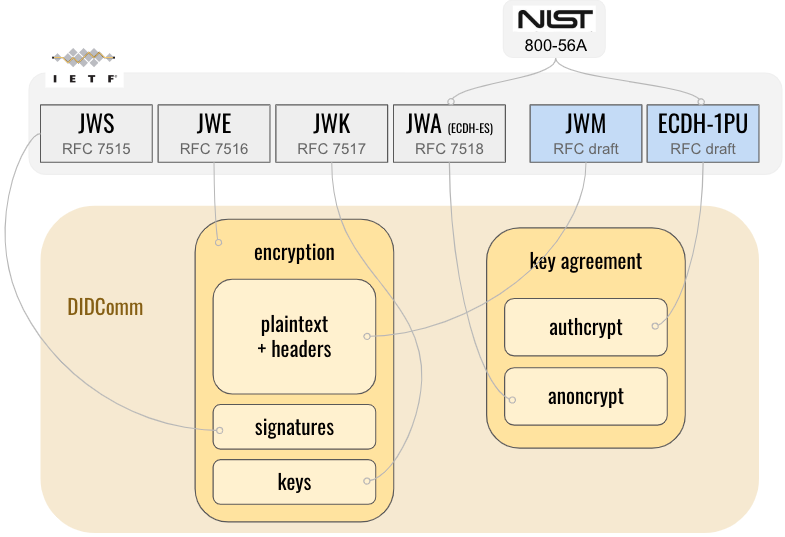
\includegraphics[width=0.7\textwidth]{related_work/didcomm_tools.png}
  \caption{Standards used in DIDComm \cite{hardman_2021}}
  \label{fig:didcomm_tools}
\end{figure}

As shown in figure \ref{fig:didcomm_tools}, DIDComm offers different approaches for key agreement encryption, namely, Authenticated Sender Encryption (\emph{authcrypt}) and Anonymous Sender Encryption (\emph{anoncrypt}). Both options are encrypted and delivered to the recipient's DID, but only \emph{authcrypt} can authenticate the sender's identity. Sending anonymous messages in social networks is not usually the case, and removing the attribution can lead to other problems \cite{martin_2022}. Nonetheless, social networks like Ask.fm\footnote{https//ask.fm} or NGL\footnote{https://ask.fun} that rely on anonymous posts could use the advantages of \emph{anoncrypt}.

DIDComm recommends using \emph{authcrypt} as the standard to provide confidentiality, message integrity, and authenticity of the sender. For this, \emph{authcrypt} requires the \emph{ECDH-1PU} proposed standard. An alternative to \emph{Authcrypt} that also complies with the required confidentiality and non-repudiation requirements is to have a nested JWT, shown in figure \ref{fig:nested_jwt}. To achieve this, the plaintext is first signed, and the resulting JWS is used as the JWE's content. The algorithm \ref{alg:nested_jwt} illustrates better the workings of this.

\begin{algorithm}[H]
  \caption{Communication example with nested JWT}
  \label{alg:nested_jwt}
    \begin{algorithmic}[1]
      \State Alice signs a plain text message using her private key \emph{sk\textsubscript{a}} and creates a \emph{(JWS)}.
  
      \State Alice encrypts the \emph{(JWS)} using Bob's public key pk\textsubscript{b} and creates a \emph{(JWE)}.
  
      \State Alice sends \emph{JWE} to Bob.
  
      \State Bob decrypts \emph{(JWE)} using his private key \emph{sk\textsubscript{b}} and obtains the \emph{JWS}
      \State Bob verifies \emph{(JWS)} using Alice's public key \emph{pk\textsubscript{a}}
  \end{algorithmic}
\end{algorithm}
  
\begin{figure}[H]
  \centering
  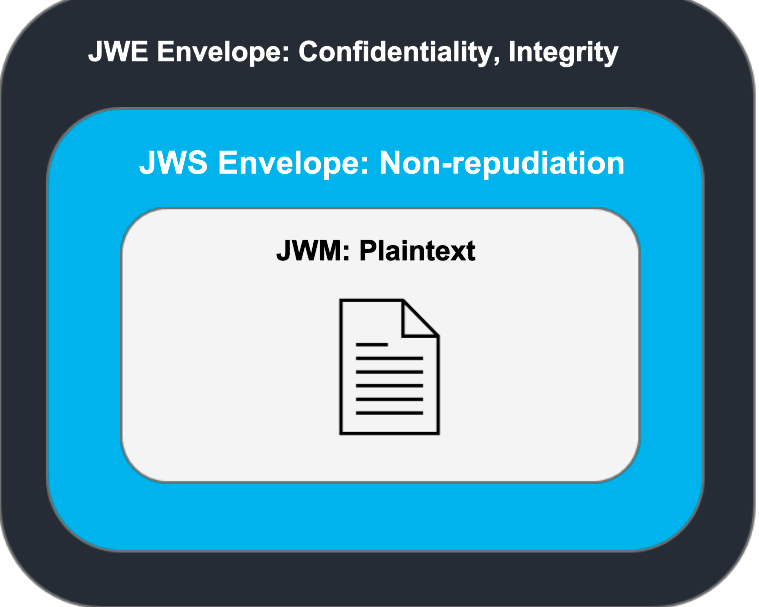
\includegraphics[width=0.5\textwidth]{related_work/nested_jwt.png}
  \caption{Nested JWT example}
  \label{fig:nested_jwt}
\end{figure}

 



% ---Left out well-known URIs. ----------
% 
% 
% \item \textbf{Change password:}
%   This endpoint origin from the proposal of the Web Application Security Working Group (WebAppSec) of the W3C. It defines a well-known URL that sites can use to make their change password forms discoverable by tools. This URL would enable software, especially password managers, to easily redirect users to the right link for them to change their password \cite{mondello_o'connor_2021}.
% 
%   \item \textbf{NodeInfo: }
%   NodeInfo is an initiative to standardize the presentation of metadata about a server operating one of the distributed social networks. The two main aims are to get greater insights into the distributed social networking user base and to provide tools that allow users to select the most suited software and server for their requirements. Mastodon is one of the implementers of this protocol, along with other federated social networks such as Diaspora, Peertube and WordPress [http://nodeinfo.diaspora.software/ ]. NodeInfo specifies that servers must provide the well-known path /.well-known/nodeinfo and provide a JRD document referencing the supporting documents via Link elements, as shown in \label{NodeInfo response example}. [http://nodeinfo.diaspora.software/protocol.html ] Accessing the hypertext reference from the JRD response will give a schematized series of metadata of the instance running the endpoint, such as NodeInfo schema version, software, protocols supported by the server, statistics and even a list of third-party services that can interact with the server via an API. Figure \label{fig:nodeinfo_response} shows the NodeInfo 2.0 schema of the Mastodon instance mastodon.social. 
% \end{itemize}
% 
% 
% \lstset{style=JSONStyle}
% \begin{lstlisting}[caption=NodeInfo response example, label=NodeInfo response example, float=h]
%   {
%       "links": [
%           {
%             "rel": "http://nodeinfo.diaspora.software/ns/schema/2.1",
%               "href": "https://example.org/nodeinfo/2.1"
%           }
%       ]
%   }
% \end{lstlisting}

% \lstset{style=JSONStyle}
% \begin{lstlisting}[language=PHP, caption=NodeInfo request]
%     GET /wel-known/nodeinfo/2.0 HTTP/1.1
%     Host: mastodon.social
% \end{lstlisting}

% \lstset{style=JSONStyle}
% \begin{lstlisting}[language=PHP, caption=NodeInfo response for mastodon.social, label=fig:nodeinfo_response, float=h]
% {
%    "version": "2.0",
%    "software": {
%        "name": "mastodon",
%        "version": "3.5.3"
%    },
%    "protocols": [
%        "activitypub"
%    ],
%    "services": {
%        "outbound": [],
%        "inbound": []
%    },
%    "usage": {
%        "users": {
%            "total": 718555,
%            "activeMonth": 61717,
%            "activeHalfyear": 178356
%        },
%        "localPosts": 36484017
%    },
%    "openRegistrations": true,
%    "metadata": []
% }
% \end{lstlisting}